\documentclass[]{article}
\usepackage{graphicx}
\usepackage{float}
\usepackage[normalem]{ulem}
\useunder{\uline}{\ul}{}

\setlength{\oddsidemargin}{.1in} %.25in
\setlength{\evensidemargin}{.25in} %.25in
\setlength{\textwidth}{6.25in} %5.75
\setlength{\topmargin}{-0.4in} %-0.4in
\setlength{\textheight}{8.5in} %8.5in

\setlength{\parindent}{0pt} %0pt
\setlength{\parskip}{0.5em} %0.5em

%opening
\title{Honeypot Threat Analysis}
\author{Alex Doolan}
\date{}


\begin{document}
	
\maketitle

\section{Introduction}

\subsection{Project Overview}

The integrity of public-facing infrastructure is constantly challenged by automated botnets seeking to compromise Secure Shell (SSH) services. While the massive volume of password brute-forcing is well-documented, a comprehensive understanding of both the specific infiltration tactics and the subsequent post-exploitation behaviour of these botnets remains critical. This project conducts a comparative analysis of these attack vectors through the deployment of a medium-interaction honeypot infrastructure.

Over a period of four weeks, three distinct instances of the Cowrie SSH honeypot (commonly referred to as "Sensors") were deployed on Amazon Web Services (AWS) cloud infrastructure. The project aimed to profile the behaviour of automated attackers by comparing generic dictionary attacks against highly targeted Internet of Things (IoT) brute-force campaigns. Crucially, the project also tested the responsiveness of threat actors to "Honeytokens" (active deception credentials). By intentionally leaking private Ed25519 SSH keys on public GitHub repositories and embedding fake AWS API keys and sensitive documents within the honeypots' simulated filesystems, this project seeks to determine if adversaries scraping public repositories and exploring compromised systems are distinct from the background radiation of standard, unsophisticated brute-force botnets.

\subsection{Motivation and Problem Statement}

Automated attacks are typically characterised as "low-skill" and "high-volume," relying on massive dictionary attacks against common usernames and passwords. Previous studies, such as those by Fraunholz et al. (2017) \cite{fraunholz2017investigation}, have successfully profiled this "background noise", establishing that the vast majority of SSH traffic is generated by unsophisticated botnets (e.g. Mirai) that do not employ evasion techniques or high-value targeting.

However, significant gaps exist in understanding the full lifecycle of these attacks - specifically, whether attacking scripts adapt to their targets during the infiltration phase, and whether their post-compromise activity varies based on the infrastructure they breach. Furthermore, with many open-source and public repositories being hosted online, the accidental leakage of secrets in these repositories has become a major vulnerability. While it is known that attackers use brute-force methods, it is less clear how quickly and effectively they monitor platforms like GitHub for secret information, whether they actively search compromised filesystems for sensitive data, and whether they then use this data in a secondary attack.

This project addresses this gap by investigating three distinct questions:

\begin{enumerate}
	\item \textbf{Baseline and IoT Profiling:} Does restricting the "attack surface" (e.g. simulating specific IoT devices versus generic servers) alter the profile or volume of the attacking botnets?
	
	\item \textbf{Post-Exploitation Behaviour:} Do the post-compromise commands executed by adversaries differ based on the specific credentials they used to successfully breach a system? Does their activity differ based on the credentials used to access the system?
	
	\item \textbf{Repo-Scraping Efficiency:} Is there an active, automated ecosystem of "sniffers" monitoring GitHub for private keys, or exploring compromised filesystems for secondary tokens? If so, does the usage of these tokens in a secondary attack indicate a higher level of sophistication or intent compared to standard brute-force attacks?
\end{enumerate}


\section{Related Work}

This section reviews the existing academic literature surrounding Secure Shell (SSH) honeypot deployment and the classification of automated attack traffic. It establishes the current understanding of "background radiation" traffic and identifies specific gaps regarding the exploitation of high-value cryptographic material compared to standard credential stuffing.

\subsection{Automated Adversaries and Credential Exploitation}

The proliferation of automated scanning tools has created a saturation of brute-force attacks against public-facing infrastructure. Research focusing on the source and complexity of the credentials used in these attacks reveals a significant disconnect between sophisticated data breaches and the actual traffic hitting SSH sensors. In their 2025 study, Rabzelj and Sedlar demonstrated that automated attackers prioritise volume over precision, relying almost exclusively on generic wordlists (e.g. "password", "123456") and factory-default IoT credentials rather than user-specific passwords \cite{rabzelj2025beyond}.

Differentiating the behaviour of these automated bots from human actors post-compromise is equally critical. Fraunholz et al. (2017) \cite{fraunholz2017investigation} deployed a medium-interaction honeypot to capture and classify session activity, finding that the overwhelming majority of successful intrusions resulted in non-interactive, pre-scripted execution, such as the immediate download of malware binaries. Their study confirmed that SSH traffic is driven by highly distributed botnets that rarely utilise network obfuscation (such as VPNs or TOR), implying a strategy of "smash and grab" where stealth is deemed unnecessary. This research establishes a clear baseline profile for standard SSH attacks: high-volume, highly distributed, and low-interaction.

\subsection{Longitudinal Behaviour and the Research Gap}

A significant challenge in honeypot research is the validity of data collected over extended periods. Munteanu et al. (2025) \cite{munteanu2025attacks} explored this in a longitudinal study of honeynet traffic, demonstrating that sophisticated botnets employ "fingerprinting" techniques to identify honeypot emulation quirks. Once a sensor is identified, its IP address is frequently blacklisted by the botnet controller, resulting in a documented "Decay Curve" where traffic volume drops significantly. Furthermore, Munteanu et al. noted a tactical shift in modern botnets toward executing exploratory commands to verify the victim's authenticity before deploying payloads.

While the reviewed literature establishes a consensus that the majority of SSH background radiation consists of low-skill, password-based botnets that exhibit predictable decay patterns, a critical gap remains regarding supply chain exploitation. Specifically, there is limited empirical research addressing the automated harvesting of leaked cryptographic keys from public repositories. It remains unclear if the profile of an attacker exploiting a leaked "Honeytoken" differs from the standard brute-force population, and whether active deception can effectively counter sensor decay by signalling value to the attacker. This project aims to address these gaps by directly comparing the behaviour of standard credential-stuffing botnets against those targeting exposed cryptographic secrets.

\section{Methodology and Experimental Design}

This section details the architecture, software selection, and experimental variables used to create the honeypots and analyse the attacks done on them.

\subsection{Host Infrastructure and Architecture}

To simulate a realistic target, the honeypot infrastructure was deployed on cloud servers. Whilst hosting it on a physical device (such as a Raspberry Pi) was considered, it would have had a large speed impact on whichever network it was running on, and would have potentially posed a real security risk if the network was misconfigured or the honeypot was somehow "broken out of" by an adversary.

Major cloud providers (such as Amazon Web Services, Microsoft Azure and Google Cloud) were preferred as their IP ranges are more likely to be targeted by automated scanning scripts, ensuring a high probability of engagement. Virtually all major cloud providers have the capability to run the infrastructure needed for this project, so the main factor in deciding which provider to use was cost. The choice was made to use Amazon Web Services (AWS) to host the honeypots. The "free tier" that AWS offers provides \$200 of free "credit", which fully covered the costs of running the honeypots, data storage and creating backup images \cite{awsfreetier}. The "Security Groups" functionality of AWS also made it easy to manage which incoming connections are accepted and from which port, preventing any adversary from attempting to connect to the "real" SSH port. This made AWS an appropriate choice for this project.

Three independent EC2 instances were created within AWS for the honeypots. The \texttt{t3.micro} tier \cite{awst3} running \texttt{Ubuntu Server} was chosen as it had the resources to run the honeypot software, and the cost was low enough to be run for 4 weeks within AWS's free credit limit. Each instance was given a unique IPv4 address to ensure that any adversary "fingerprinting" a sensor as a honeypot would not affect the traffic the other sensors received.

\subsection{Honeypot Software Selection}

When selecting the honeypot software, the primary consideration was the level of interaction required to capture meaningful attacker behaviour. This needed to be done without introducing unacceptable security risks, and needed to be runnable by the \texttt{t3.micro} instance.

Low-interaction honeypots, which merely open a port and record login attempts, were considered but quickly deemed insufficient for this project. Because they do not provide a simulated shell, adversaries disconnect immediately after authenticating, preventing the observation of any post-compromise behaviour. On the other hand, high-interaction honeypots, which provide an attacker with a fully functional operating system, present a potential risk; if not properly isolated, they can be compromised and used to launch real attacks against third-party networks.

The decision was therefore made to use a medium-interaction honeypot (MIHP), and Cowrie \cite{cowrie} was chosen to achieve this. As research discussed previously notes, Cowrie is the latest SSH MIHP with respect to community activity and support \cite{fraunholz2017investigation}, and as recently as 2025 has been regarded as one of the most widely used MIHPs for the malicious activity analysis this project is trying to achieve \cite{munteanu2025attacks}. 

Cowrie is an open-source MIHP built with Python that supports both SSH and Telnet. It emulates a standard UNIX filesystem, allowing attackers to "authenticate" and interact with a simulated environment. This capability is crucial for analysing the post-compromise activity of adversaries, allowing any commands run and any malicious binaries downloaded to be captured. Furthermore, Cowrie supports extensive and customisable logging capabilities, and can be configured to send logs to a central database.

It was configured to record both the initial authentication attempts (capturing usernames, passwords, and any SSH keys used) and the subsequent session data (recording keystrokes and executed commands). To make analysis efficient, Cowrie was configured on each sensor to forward all event data to a centralised MariaDB database, this was hosted on sensor 1 (see 3.3.1).

\subsection{Sensor Configuration and Experimental Variables}

To accurately profile attackers and address the specific questions regarding public repository leaks, three AWS instances were configured, each with their own Cowrie instance installed, and each with their own distinct authentication profiles. The decision was made to have three instances as deploying a singular instance would make distinguishing between generic background scanning, IoT-specific targeting, and the exploitation of leaked keys far more difficult.

\subsubsection{Honeypot 1}

Honeypot 1 was established as the control sensor. It was configured to emulate a generic Ubuntu server and accepted a broad dictionary of common, weak passwords. The objective of this sensor was to capture low effort brute attacks, establishing a baseline of high-volume, unsophisticated attacks against which the other sensors could be compared.

This sensor also hosted the MariaDB database, collecting data from all three sensors.

\subsubsection{Honeypot 2}

Honeypot 2 was designed to simulate a vulnerable embedded device. Instead of accepting generic passwords, its authentication profile was strictly limited to a predefined list of known default credentials (such as those commonly used by the Mirai and Gafgyt botnets). This was implemented to filter out generic dictionary attacks and isolate traffic from botnets seeking to specifically target consumer routers and IoT devices.

\subsubsection{Honeypot 3}

Honeypot 3 was the experimental sensor for testing whether credentials scraped from public GitHub repositories are being used to gain unauthorised access to devices. To eliminate standard attacks, password authentication was completely disabled on this sensor. Instead, the server was configured to only accept SSH keys, including the keys that were purposefully "leaked" on the public GitHub repository. This configuration would test whether the leaked keys would be used by scrapers to attempt a real attack, and if so, allow the "Time-to-Compromise" of the leaked keys to be measured. It could then also be used to analyse post-compromise activity, and compare this activity to that of botnets attacking sensors 1 and 2.

\subsection{Data Extraction and Analysis Pipeline}

Upon the conclusion of the four-week data collection phase, the database required processing to extract and analyse attacker behaviour. To allow easy reproducibility, the data analysis was constructed using Jupyter Notebooks \cite{jupyter} written in Python. The choice of Jupyter Notebooks enabled the code to be displayed, explained and runnable on the same page. It facilitated a step-by-step "walkthrough" of the findings, rather than just giving the code with the end result. It is also an industry standard for data science and analysis work, and so was the obvious choice for this project.

Within the code, the data manipulation processes were performed using the Pandas \cite{pandas} library. Pandas was selected due to it's high performance and efficiency in handling large, structured datasets. It is also well maintained and developed, making it a suitable choice for this project.

To visibly show the results of the analysis with graphs and charts, the Matplotlib \cite{Hunter:200:matplotlib} library was used. Matplotlib is a popular library for creating data visualisations in Python, and is very commonly used in industry and academia for the data analysis this project attempts to achieve.

\section{Implementation}

This section details the practical deployment of the honeypot infrastructure, outlining the technical configurations, the deployment of the Cowrie software and the remediation of the challenges encountered during the collection of the data.

\subsection{Cloud Environment and Network Configuration}

The foundation of the project was established by creating three independent virtual machines (VMs) within the Amazon Web Services (AWS) environment. Three EC2 instances were launched using the \texttt{t3.micro} hardware profile, with the latest LTS release of Ubuntu Server chosen as the host operating system. For additional security, these VMs were set up to require an RSA key for authentication.

Careful network configuration was required to secure the host operating system of each VM whilst simultaneously exposing the honeypot to the internet. By default, the legitimate SSH daemon (\texttt{sshd}) on Ubuntu Server listens on port 22. Leaving the legitimate shell on this port would interfere with honeypot collection and so needed to be changed. Therefore, the legitimate SSH service needed to be reconfigured within the \texttt{/etc/ssh/sshd\_config} file to listen on different port. Any high, unused port could have been used, but port 8022 was used for the three VMs in this project.

As an extra security measure, a single AWS Security Group was made and assigned to all three VMs, which acts as a network-level firewall. In the first instance, this was configured to strictly limit inbound access to port 8022 to my home IP address, and block any other connections to any other ports. The security group rules would later be updated as the setup progressed.

With the SSH port changed and the security group implemented, the VMs were prepared for the honeypot software. As a security measure, Cowrie is designed to run as an unprivileged user, and so doesn't have the permissions to bind to privileged network ports (ports below 1024). Because of this, Cowrie listens on port 2222 (SSH) and 2223 (Telnet) by default, and the user needs to configure the operating system to send connections from the standard SSH and Telnet ports to Cowrie's SSH and Telnet ports. To do this, a Network Address Translation (NAT) routing rule was added to each VM using the \texttt{iptables} utility. A \texttt{PREROUTING} rule was configured to take all inbound TCP traffic to ports 22 and 23 and redirect it to ports 2222 and 2223 respectively.

\subsection{Honeypot Deployment and Configuration}

Following the preparation of the host infrastructure, the Cowrie honeypot software was deployed onto each of the three EC2 instances. First by creating a dedicated "cowrie" user, then cloning the repository, and then by setting up a Python virtual environment to prevent any version conflicts. It's dependencies were then installed using the provided \texttt{requirements.txt} file.

Once Cowrie was installed on the three instances, the different experimental variables explained in Section 3.3 were implemented by modifying Cowrie's primary configuration file (\texttt{cowrie.cfg}) and its authentication rules (\texttt{userdb.txt}).

Copies of the full \texttt{userdb.txt} authentication rules for Honeypots 1 and 2 can be found on the project GitLab in the \texttt{/credentials} folder.

\subsubsection{Honeypot 1}

For Honeypot 1 (the control sensor), the implementation required minimal deviation from  a standard deployment. The \texttt{cowrie.cfg} file was configured to listen on the redirected port 2222, and the \texttt{userdb.txt} file was populated with a broad, generic dictionary of commonly abused usernames and passwords, with only extremely basic combinations like "root:root", "root:123456" and "root:honeypot" disallowed (to prevent botnets "fingerprinting" the machine as a honeypot). This permissive configuration ensured that the sensor would capture a high volume of unsophisticated attacks.

\subsubsection{Honeypot 2}

The implementation of Honeypot 2 required a more restrictive approach to entice adversaries attempting to attack vulnerable IoT devices. The generic entries within the \texttt{userdb.txt} file were completely removed. In their place, a highly specific list of default credentials known to be utilised by IoT-targeting botnets, such as Mirai and Gafgyt, was inserted (e.g. \texttt{root:xc3511}, \texttt{root:vizxv}). By hardcoding these limitations into the authentication rules, the honeypot effectively filtered out generic brute-force attempts; an attacker could only successfully instantiate a session if they were utilising a dictionary containing known IoT credentials.

\subsubsection{Honeypot 3}

Honeypot 3 represented the most complex configuration, as it required shifting the authentication mechanism from passwords to cryptographic keys. Within the \texttt{cowrie.cfg} file of the third instance, the \texttt{auth\_password} directive was explicitly set to \texttt{false}, entirely disabling password attacks. Concurrently, the \texttt{auth\_publickey} directive was enabled. A limitation of Cowrie is that the \texttt{auth\_publickey} setting is an "all or nothing" directive, meaning that Cowrie either accepts all keys or it accepts no keys. There is no feature in Cowrie at the time of writing that enables you to insert specific keys for authentication. However, it will still log a hash of any keys used, which gives enough information to test if the leaked keys are being used.

\subsubsection{Public GitHub Repositories}

Three \texttt{Ed25519} key pairs were generated and the private keys intentionally uploaded to three GitHub repositories (private when first created, but purposefully set to public at the same time the honeypots were started). The three repositories were named \texttt{server-automation-scripts} \cite{server-automation-scripts}, \texttt{dotfiles-local} \cite{dotfiles-local} and \texttt{legacy-db-migration} \cite{legacy-db-migration} and were created under the same fresh GitHub account \newline(\texttt{deploybackup2025}). All three were created to replicate seemingly private repositories that were "accidently" leaked, and all contained the IP address associated with the instance running honeypot 3 somewhere in the repository. 

\texttt{dotfiles-local} contained its key within the \texttt{.ssh/id\_ed25519} file, with the server IP in \texttt{.ssh/config}. \texttt{server-automation-scripts} contained its key and the server IP address inside a .json file \newline(\texttt{config/production.json}). However, \texttt{legacy-db-migration} was slightly different, the key and server IP was purposefully committed and then removed in a subsequent commit, attempting to replicate a developer that either didn't realise or forgot that the code changes in previous commits can be viewed publicly. The purpose of these slight differences was to see if they had any impact on the ability of scrapers to find the IP and key, and hence see if that had any impact on the volume of attacks.

The three GitHub repositories can be viewed via the citations above. The links are also at the top of the \texttt{README.md} on the project GitLab.

\subsubsection{Fake Filesystem and Insertion of Honeytokens}

Once the authentication set-up for each of the honeypots was complete, the next stage was to create the fake filesystem that attackers would see when a honeypot was successfully logged into. Cowrie by default gives a standard linux filesystem, but this was adjusted to include some traceable "honeytokens". Honeytokens are fake file resources that are designed to be attractive to attackers, the files themselves don't contain anything real, but when opened or used they trigger an alert that signifies unauthorised use \cite{honeytokens}.

The free "Canarytokens" tool by Thinkst Applied Research \cite{canarytokens} was used to generate six tokens, three were fake AWS API keys, and three were fake Microsoft Excel spreadsheets. One token of each type was used for each of the three honeypots. The tokens were setup to send an email to a fresh account created for the project if they were triggered. The AWS token would be triggered if an adversary attempted to use the API key. The Excel document token would be triggered if the file was opened.

The Cowrie file system contains two parts: a pickle file (\texttt{fs.pickle}) which mostly contains metadata for the files, and the \texttt{honeyfs} directory, which holds the contents of user created files. For the contents of the file to be shown to an attacker, the file first needs to be placed in the \texttt{honeyfs} directory, and then an associated entry needs to be made to \texttt{fs.pickle}. 

For each of the three honeypots the layout of the honeytokens was the same. Within \texttt{honeyfs}, the fake AWS keys were inserted into a newly created \texttt{.aws} folder contained within the home directory of each user (including \texttt{root}), the AWS tokens were given the file name \texttt{credentials}. The Microsoft Excel tokens were inserted directly into the home folder of each user (including \texttt{root}), and were given the name \texttt{Server\_Inventory.xlsx}, to give the impression that the file was sensitive. Once added to \texttt{honeyfs}, entries for the files were then added to \texttt{fs.pickle} using Cowrie's file system editor tool \texttt{fsctl}.

Some other minor changes were made to the filesystem to make it more realistic and remove things that could "fingerprint" the instances as honeypots. Cowrie by default has the user "\texttt{phil}" in it's filesystem, this could quickly identify the system as a Cowrie honeypot, so the user was removed. Home folders were also made for each of the usernames listed in the authentication files, so adversaries would be "logged in" to the expected folder. Within each users home folder, \texttt{.bashrc}, \texttt{.profile}, and \texttt{.bash\_logout} entries were also added to \texttt{fs.pickle} for realism.

\begin{figure}[H]
	\centering
	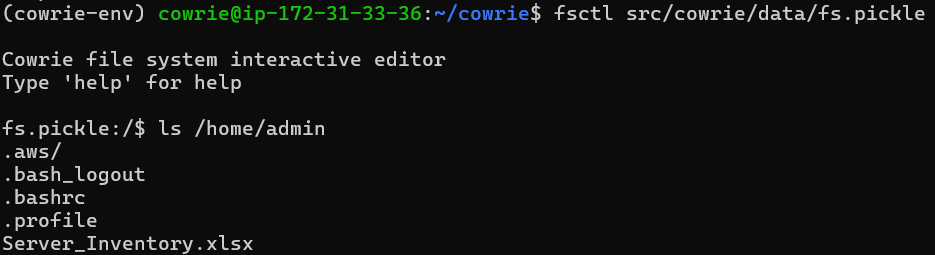
\includegraphics[width=0.65\textwidth]{hp1_admin_fake_file_system.png}
	\caption{\texttt{fs.pickle} entry for the \texttt{admin} users home directory - Honeypot 1}
\end{figure}

\subsection{Centralised Collection of Logs}

To allow the data collected to be efficiently queried in the analysis stage, a central database was used. MariaDB, an open source relational database management system based on MySQL \cite{mariadb}, was installed on the Honeypot 1 instance to collect the attack data from all three honeypots. A new database named \texttt{cowrie} was made, and then \texttt{cowrie.cfg} was modified on all three instances to uncomment the \texttt{output\_mysql} module, enabling the database logging. The \texttt{host}, \texttt{database}, \texttt{username} and \texttt{password} fields within the \texttt{output\_mysql} module then needed to be modidied, inserting the database and user name (both \texttt{cowrie}) and the database password (created when the database was made). For the host field, \texttt{localhost} was entered for honeypot 1 (As HP1 is hosting the database). For honeypots 2 and 3, the private IP of honeypot 1 was entered (to tell HP2 and HP3 to send their logs to HP1). The AWS security group was then updated to allow honeypot 1 to receive data from honeypots 2 and 3.

\subsection{Operational Challenges and Remediation}

The primary operational constraint of the project was the hardware limitation of the AWS \texttt{t3.micro} instances, which are provisioned with only 1GB of RAM. While this is generally sufficient for a baseline Ubuntu installation with Cowrie running in the background, the memory Cowrie uses expands significantly during high-volume attack spikes. When a botnet aggressively attacks a sensor, the connection handling and (in the case of honeypot 1) intensive database writing can exhaust the available memory. 

This extensive use of memory was an oversight that was not realised straight away, and lead to what was the largest setback the project faced. All three sensors were initially started on 21st December 2025. However, around 10 days in it was noticed that Cowrie on honeypots 1 and 2 were no longer running. By using the \texttt{dmesg} (diagnostic message) utility and filtering for the word "kill" (\texttt{dmesg | grep -i "kill"}), it was quickly identified as an "Out of memory" crash for both honeypot 1 and 2. As Cowrie doesn't have a graphical user interface, it relies on running the \texttt{cowrie status} command to check it is still running, and so a crash like this could easily be missed.

To fix this a "swap file" was used, which effectively increases the "virtual memory" the OS has available beyond the physical RAM. A 5GB swap file was created. First by creating the file with \texttt{fallocate}, then given exclusively root permissions, marking the file as swap space with \texttt{mkswap} and finally turning it on with \texttt{swapon} \cite{swapfile}. This process was followed for all three honeypots.

Additionally, as a precaution, a script was created to check if Cowrie was running every 30 minutes, and restart Cowrie if it had crashed. This was done quite easily using the cron job scheduler. A \texttt{start\_cowrie.sh} script was made, containing the commands to go to the \texttt{/home/cowrie/cowrie} directory, activate the Python virtual environment, and start Cowrie. A new line was then added to the \texttt{cowrie} users crontab, instructing the \texttt{start\_cowrie.sh} script to be ran every 30 minutes.

Whilst honeypots 1 and 2 crashing without being noticed was a setback time-wise, both honeypots were restarted with the above fixes in place on 3rd January 2026, and both completed their 4 week data collection with no further crashes.

\section{Results and Analysis}

This section presents a summary of the primary findings from the four-week collection period. All data processing and visualisation was done with Python, using the Pandas and Matplotlib libraries. Whilst this section highlights the most significant findings, the full analysis (including all code), can be found by viewing the Jupyter Notebooks found in the \texttt{notebooks} folder of the project GitLab. The code and the results can be \textit{viewed} directly from the notebooks without any setup. However, if you want to \textit{run} the code, you will need to set up a copy of the database on your local machine, full instructions on how to do this are in the GitLab \texttt{README} file.

\subsection{Traffic Distribution and Attack Volume}

Over the course of the deployment, the honeypot infrastructure recorded a large volume of automated traffic. During the active window of the sensors (03-01-2026 to 01-02-2026 for sensors 1 and 2, 21-12-2025 to 18-01-2026 for sensor 3), the sensors logged a combined total of 2,911,987 connections.

However, the traffic targeting the experimental leaked GitHub key sensor (Sensor 3) gave a contrasting result. Despite running for a full four-week period and having the corresponding SSH keys intentionally leaked on public GitHub repositories, Sensor 3, despite receiving 13731 connections, recorded 0 successful authentications.

\begin{table}[H]
	\centering
	\caption{Breakdown of Total Connections and Successful Logins by Sensor}
	\begin{tabular}{|c|c|c|c|c|}
		\hline
		Sensor & \multicolumn{1}{l|}{Connections} & \begin{tabular}[c]{@{}c@{}}Connections as a \% of \\ Total Connections\end{tabular} & Successful Logins & \begin{tabular}[c]{@{}c@{}}Successful Logins as a \% of \\ Sensor Connections\end{tabular} \\ \hline
		1      & 2,474,030                        & 84.96                                                                               & 563,965           & 22.80                                                                                      \\ \hline
		2      & 424,226                          & 14.57                                                                               & 251,283           & 59.23                                                                                      \\ \hline
		3      & 13,731                           & 0.47                                                                                & 0                 & 0                                                                                          \\ \hline
		Total  & 2,911,987                        & 100                                                                                 & 815,248           &                                                                                            \\ \hline
	\end{tabular}
\end{table}

%\begin{figure}[H]
%	\centering
%	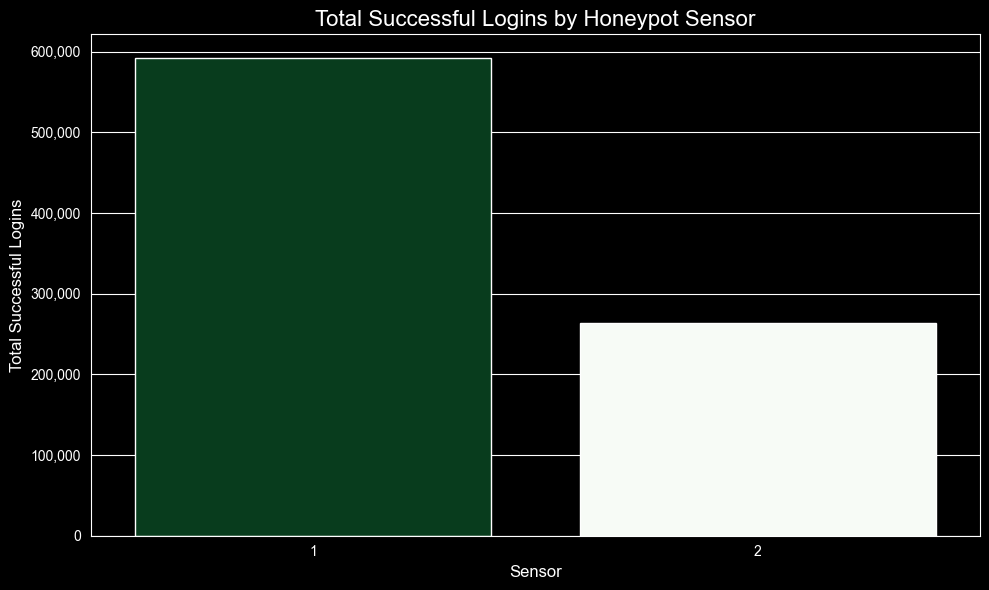
\includegraphics[width=0.8\textwidth]{successful_logins_by_sensor.png}
%	\caption{Total Successful Logins by Honeypot Sensor}
%\end{figure}

Whilst technically a null result, the lack of successful logins on Sensor 3 gives an insight into how automated attackers operate. It demonstrates that they are unsophisticated, and rely purely on scanning scripts that attempt to brute force passwords from dictionaries. In fact, the only indication that the keys were "scraped" at all was from an automated email received from GitGuardian's GitHub Public Monitoring Tool \cite{gitguardian}, which warned that the secrets were public. If any of the keys were stolen by a malicious scraper, they were not then subsequently used in a targeted attack on honeypot 3.

To compound the evidence that the attacks on the honeypots were unsophisticated, the "honeytokens" added to the honeypot filesystems (see 4.2.5) did not get used at all. The email account set up to receive any notifications of the excel document being opened or the AWS API key being used received 0 alerts. This evidence implies that the attackers that connected were not interested in searching the filesystem for any sensitive files, they ran their pre-configured script and then disconnected.

\subsection{Credential Analysis}

During the active window of sensors 1 and 2, 2,607,894 authentication attempts were recorded. The overall data suggested that attackers attempted to use a mixture of both basic credentials (such as \texttt{root:root}) and credentials related to specific devices (such as \texttt{root:vizxv}).

A targeted analysis of Sensor 2 provided a deeper understanding of how botnets target vulnerable IoT devices. Sensor 2 captured 312,373 authentication attempts, and the credentials used highlight the active targeting of embedded systems, including:

\begin{itemize}
	\item Dahua and XiongMai IP Cameras (\texttt{root:xc3511}, \texttt{root:vizxv})
	\item Huawei HiSilicon Chips (\texttt{root:hi3518})
	\item ZTE Routers (\texttt{root:zju68})
\end{itemize}

A comparative analysis of sensors 1 and 2 across the top 30 credentials for each was also done. This showed the overlap in the credentials used was only 33.3\%. The low overlap could suggest that the honeypots were targeted by distinct botnets, each relying on slightly different dictionaries. On the other hand, this low overlap could be caused by Sensor 1 accepting more basic credentials; if an automated script successfully authenticates early in its execution using a basic password (like \texttt{root:1234}), it will immediately stop guessing, thereby preventing the IoT-specific credentials further down its list from being logged on Sensor 1.

Interestingly, many of the top credentials attempted on Sensor 1 were still IoT-specific credentials, despite the fact that Sensor 1 will accept far more basic ones. This suggests that the scripts the attackers are using do not adapt or "learn" from their environment. Rather than adjusting their guesses based on the specific rules of the honeypot, they blindly cycle through their pre-programmed list. This indicates that bots act as singular "dumb" workers rather than in coordination with each other. They do not appear to share authentication information with other nodes in the botnet to optimise attacks. This further compounds the evidence in 5.1 that these adversaries rely on pure attack volume rather than sophisticated, intelligent tactics.

\begin{figure}[H]
	\centering
	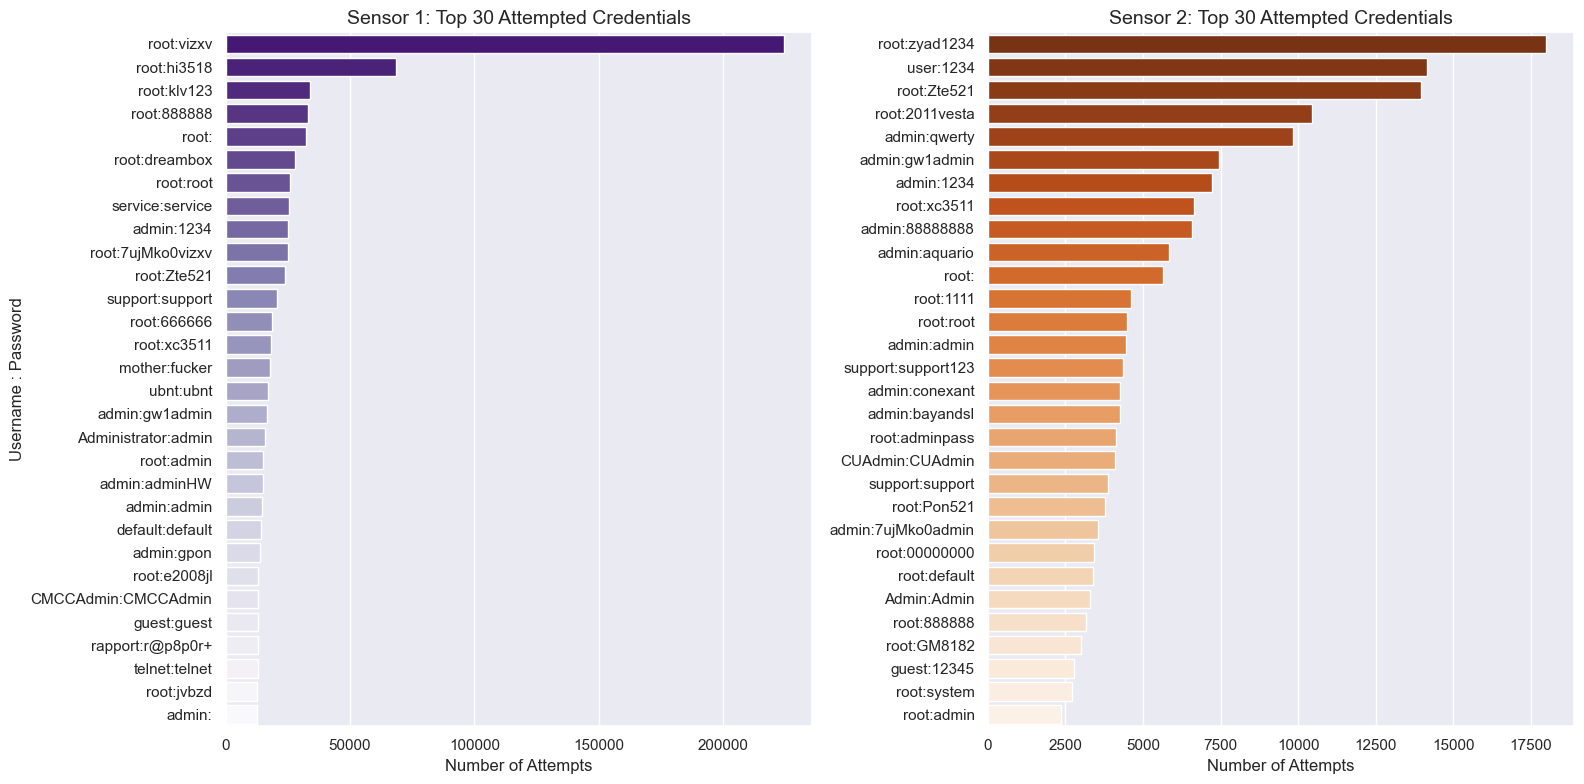
\includegraphics[width=1\textwidth]{top_credentials_by_sensor.png}
	\caption{Top 30 Attempted Credentials on Sensor 1 (left) and Sensor 2 (right)}
\end{figure}

\subsection{Post-Exploitation Activity}

After filtering the dataset for successful authentications, the post-compromise activity of the attacker was analysed. During the active window, the sensors recorded a total of 13,397,852 shell commands executed by attackers after gaining access.

When analysing the most frequently executed commands across sensors 1 and 2, an interesting anomaly emerged: the top five commands (\texttt{shell}, \texttt{system}, \texttt{start}, \texttt{config terminal}, and \texttt{linuxshell}) had almost identical execution counts of approximately 1.61 million each. As well as this, other groups of commands also showed near-identical execution counts, with \texttt{sh}, \texttt{enable} and \texttt{su} for example all being executed approximately 807,300 times. This perfectly illustrates the automated behaviour of botnets. Because many embedded devices drop users into restricted configuration menus rather than a standard bash terminal, botnets appear to be programmed to send a hardcoded sequence of universal "escape" commands.

Once a functional shell is accessed, the scripts immediately use network utilities like \texttt{wget} or \texttt{curl} to pull down malware payloads. By parsing the raw command strings for URLs and IP addresses, 952 unique malicious servers were identified as drop-zones for this malware.

Interestingly, a comparative analysis of the commands run between Sensor 1 and Sensor 2 revealed that their post-compromise command profiles were nearly identical in both execution order and proportional frequency (see figure 3). This suggests that even when non-IoT-specific credentials are used to gain access to the honeypots, the attack scripts still appear to run commands that are designed to specifically target IoT devices, suggesting that vulnerable IoT devices are the primary target of these automated attacks. This also compounds the earlier evidence that these adversaries are unintelligent and rigid, they don't appear to change their behaviour in any way based on the credentials used to access the system.

\begin{figure}[H]
	\centering
	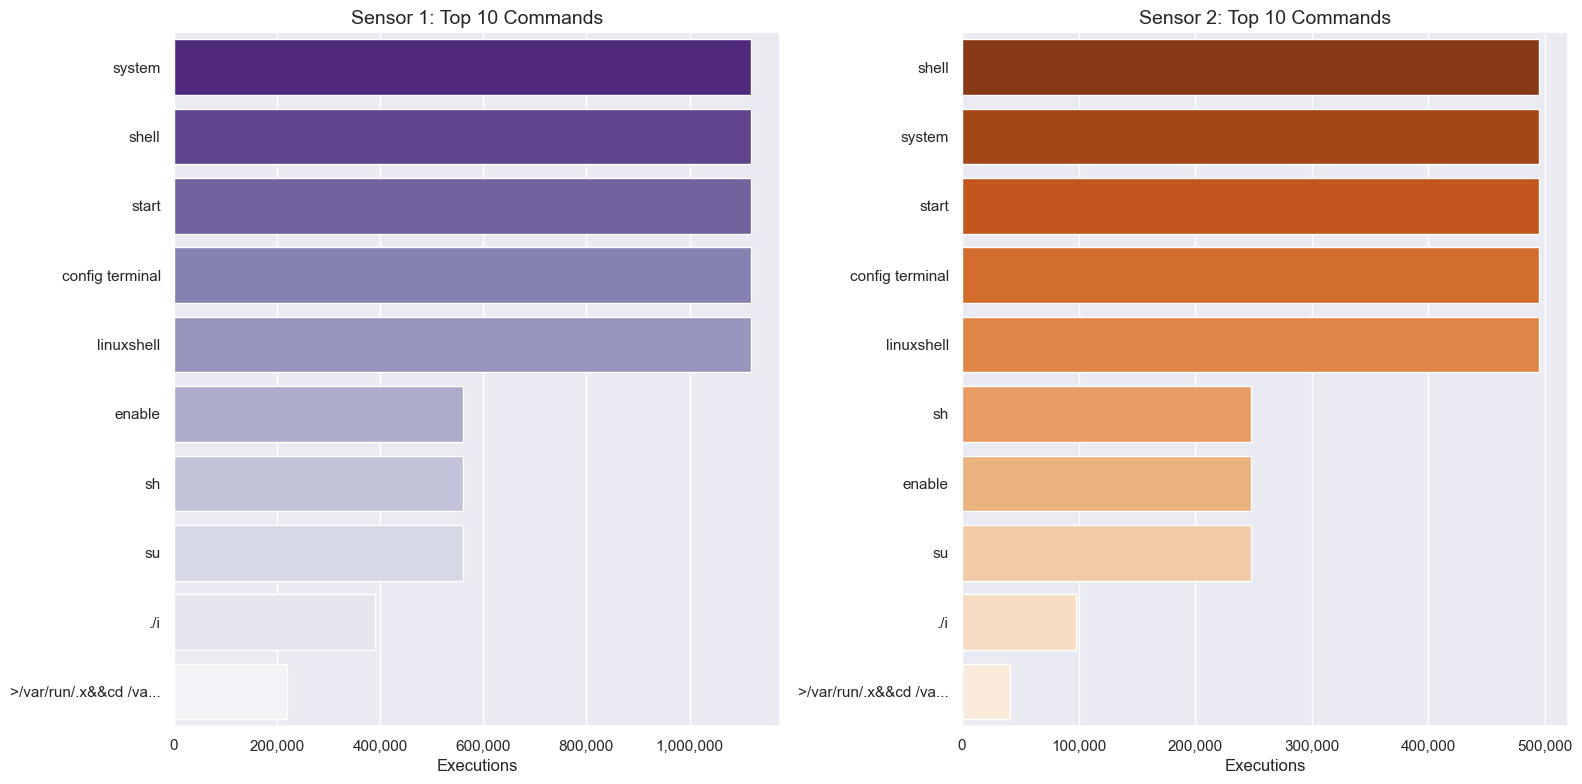
\includegraphics[width=1\textwidth]{top_commands_both_sensors.png}
	\caption{Top 10 Commands Executed on Sensor 1 (left) and Sensor 2 (right)}
\end{figure}

\section{Conclusion}

This project deployed a comparative honeypot infrastructure to profile automated adversaries and evaluate the efficacy of leaked secrets being used for secondary attacks. The findings provide evidence that the background radiation of traffic is overwhelmingly dominated by high-volume, unsophisticated attackers relying on pre-programmed scripts. Over four weeks, the sensors logged over 2.9 million connections and 13.3 million post-exploitation shell commands, highlighting the scale of these automated attacks.

The credential analysis revealed that infiltration is specialised but rigid. Distinct botnets appear to utilise password dictionaries tailored to vulnerable IoT infrastructure, yet they act as singular "dumb" workers that do not dynamically adapt or learn from the honeypot's responses. The post-compromise exploitation appeared to be highly homogenised. Regardless of the credentials used to breach the system, attackers universally deployed identical, hardcoded sequences of "escape" commands to bypass restricted menus and utilised utilities like \texttt{wget} or \texttt{curl} to download secondary malware payloads.

Finally, the leaked secrets experiments yielded interesting insights. The total absence of traffic targeting the leaked GitHub SSH keys, alongside the completely untouched internal Canarytokens (fake AWS keys and Excel documents), demonstrates that these automated adversaries do not engage in intelligent repository scraping or manual filesystem exploration for sensitive data. Ultimately, this project confirms that modern automated attacks largely target vulnerable IoT devices, and prioritise indiscriminate speed and volume over sophisticated, targeted intrusion tactics.


\bibliographystyle{ieeetran}
\bibliography{References}
\end{document}

%Things I would of done differently: made sensor 2's file system emulate that of an IoT device
